% Created 2025-04-11 Fri 00:22
% Intended LaTeX compiler: pdflatex
\documentclass[11pt]{article}
\usepackage[utf8]{inputenc}
\usepackage[T1]{fontenc}
\usepackage{graphicx}
\usepackage{longtable}
\usepackage{wrapfig}
\usepackage{rotating}
\usepackage[normalem]{ulem}
\usepackage{amsmath}
\usepackage{amssymb}
\usepackage{capt-of}
\usepackage{hyperref}
\usepackage[slovene]{babel}
\usepackage[]{babel}
\usepackage{float}
\author{Nikola Brković}
\date{\today}
\title{XMPP}
\hypersetup{
 pdfauthor={Nikola Brković},
 pdftitle={XMPP},
 pdfkeywords={},
 pdfsubject={},
 pdfcreator={Emacs 29.4 (Org mode 9.6.15)}, 
 pdflang={Slovene}}
\begin{document}

\maketitle

\section{Namen protokola}
\label{sec:org207ef1e}

XMPP je protokol, namenjen izmenjavi strukturiranih podatkov v
približno realnem času med dvema ali več entitetami
(Peter Saint-Andre, 2011). Kratica XMPP pomeni \emph{Extensible Messaging and
Presence Protocol}, oziroma v slovenščini - razširljiv protokol za
sporočanje in prisotnost.

Čeprav je v teoriji XMPP splošno-namenski protokol za izmenjevanje
sporočil, v praksi se pa največkrat uporablja za hipno sporočanje
(\emph{ang.} \emph{instant messaging} oziroma \emph{IM}) in aplikacije, ki ponujajo
funkcionalnost klepetanja.

\section{Arhitektura protokola}
\label{sec:orgfec76b4}

Pri arhitekturi protokola so se ustvarjalci protokola XMPP zgledovali
po protokolu SMTP. Udeleženci v protokolu XMPP so povezani v
porazdeljenem omrežju. Vsak udeleženec je bodisi strežnik bodisi
klient. Poznamo tudi entitete, ki jim pravimo viri, ki pripadajo
določenemu uporabniku. Komunikacija lahko poteka ali med strežniki ali
med strežniki in klienti. En klient je lahko povezan na samo en
strežnik in z drugimi klienti lahko komunicira le posredno prek (enega
ali več) strežnikov.

Vsaka entiteta ima svoj unikatni identifikator oziroma naslov,
kateremu pravimo \emph{Jabber ID} oziroma \emph{JID}.

Za strežnike velja, da je njihov JID enak njihovi domeni
(npr. \texttt{jabber.si}).  JID-ji uporabnikov so oblike
\texttt{<uporabnik>@<strežnik>} (npr. \texttt{julija@jabber.si}), pri čemer je
strežnik tisti strežnik, na katerem je račun uporabnika
prijavljen. Unikatne naprave ali viri, ki so vezane na določenega
uporabnika imajo JID oblike \texttt{<uporabnik>@<strežnik>/<vir>}
(npr. \texttt{julija@jabber.si/prenosnik}).

\section{Scenarij komunikacije}
\label{sec:org5c2cec1}

Ko govorimo o komunikaciji med uporabniki, lahko govorimo o
komunikaciji med uporabniki, prijavljenimi na istem strežniku, kot je
prikazano na Sliki \ref{fig:org8b57255}, ali med uporabniki, prijavljenimi
na različnih strežnikih, kot je prikazano na Sliki \ref{fig:org5018eae}.

\begin{figure}[H]
\centering
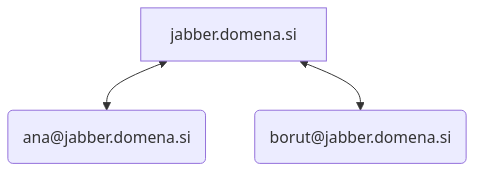
\includegraphics[width=.9\linewidth]{images/local-server.png}
\caption{\label{fig:org8b57255}Komunikacija med uporabniki na istem strežniku}
\end{figure}

\begin{figure}[H]
\centering

\includegraphics[width=.9\linewidth]{images/cross-server.png}
\caption{\label{fig:org5018eae}Komunikacija med uporabniki na različnih strežnikih}
\end{figure}

\section{Opis specifikacije}
\label{sec:orgf50d394}

Protokol XMPP je opisan v več ločenih RFC-jih:

\begin{itemize}
\item \href{https://datatracker.ietf.org/doc/rfc6120/}{Extensible Messaging and Presence Protocol (XMPP): Core} (v
nadaljevanju: \emph{XMPP-CORE})
\item \href{https://datatracker.ietf.org/doc/rfc6121/}{Extensible Messaging
and Presence Protocol (XMPP): Instant Messaging and Presence} (v
nadaljevanju: \emph{XMPP-IM})
\item \href{https://datatracker.ietf.org/doc/rfc7622/}{Extensible Messaging and Presence Protocol (XMPP): Address Format} (v
nadaljevanju: \emph{XMPP-ADDR})
\end{itemize}

Specifikacija XMPP-CORE predstavlja minimalno potrebno funkcionalnost
za strežnik oziroma klient, ki implementira XMPP. Poleg teh treh
RFC-jev je velik del funkcionalnosti XMPP v razširitvah, ki jim
pravimo \emph{XEP}-ji (\emph{XMPP Extension Protocols}). Implementacije
protokola XMPP (strežniki, klienti) implementirajo le določene XEP-je
in svoje zmožnosti oglašujejo drugim entitetam.

\subsection{XMPP-CORE}
\label{sec:org8e89edd}

V tem RFC-ju je definirano:

\begin{itemize}
\item vzpostavljanje in rušenje povezave med udeleženci v protokolu,
\item tri osnovne vrste sporočil: \texttt{<message/>}, \texttt{<presence/>} in \texttt{<iq/>}
(definirane so le vrste sporočil, struktura sporočil je pa opisana v
XMPP-IM)
\item vrste napak,
\item ter atribute sporočil. Najbolj pomembni atributi so \texttt{from}, \texttt{to} in
\texttt{id}, ki identificirata pošiljatelja sporočila, prejemnika sporočila
ter unikatni identifikator toka.
\end{itemize}

Dve entiteti, ki želita komunicirati po protokolu XMPP morata
vzpostaviti trajno povezavo po protokolu TCP, kateri pravimo \emph{tok XML}
(ang. \emph{XML stream}). Tok je sestavljen iz posameznih sporočil, katerim
pravimo \emph{stance XML} (ang. \emph{XML stanzas}). Tako posamezne stance kot
tudi celoten tok morajo predstavljati sintaksno veljavno besedilo
formata XML. Primer toka je prikazan v \href{https://xmpp.org/rfcs/rfc6120.html\#streams-fundamentals}{specifikaciji XMPP-CORE, pod
razdelkom "4.1 Stream Fundamentals"}. (Peter Saint-Andre, 2011)

Pri vzpostavitvi toka se lahko udeleženca dogovorita za šifriranje
toka s protokolom TLS, ali zahtevata avtentikacijo po protokolu SASL,
vendar je ta funkcionalnost izven obsega tega poročila.

\subsection{XMPP-IM}
\label{sec:org0f7302d}

Ta specifikacija predstavlja razširitev osnovne specifikacije, in
predpostavlja, da so entitete, udeležene v protokolu, že vzpostavile
povezavo po protokolu opisanem v XMPP-CORE.

XMPP-IM omogoča povezovanje z drugimi uporabniki oziroma kontakti. V
žargonu XMPP pravimo seznamu kontaktov \emph{spisek} (ang. \emph{roster}). Vsak
uporabnik ima svoj lastni zasebni spisek. Spisek je shranjen na
strežniku, na katerega je uporabnik prijavljen. Vnose v spisek
dodajamo in odstranjujemo z uporabo sporočil vrste \texttt{<iq/>}.

XMPP-IM omogoča tudi naročanje na prisotnost drugih uporabnikov
(ang. \emph{presence subscription}). Recimo, da se je France naročil na
Julijino prisotnost. Če Julija strežniku sporoči, da se je njena
prisotnost spremenila, bo strežnik Franceta obvestil o Julijini novi
prisotnosti. Ta obvestila se prenešajo tudi med različnimi strežniki.

Definiran je tudi koncept klepetalnih sej (ang. \emph{Chat Session}). Med
dvema entitetoma obstaja lahko ena seja, vrste \texttt{chat}. Omogočeni so
pa tudi skupinski klepeti - seja vrste \texttt{groupchat}. Informacija o
klepetalni seji je del metapodatkov sporočila vrste
\texttt{<message/>}. (Peter Saint-Andre, 2011a)

\subsection{XMPP-ADDR}
\label{sec:org1b92f2e}

Specifikacija XMPP-ADDR določa, kako so črke izven kodirne tabele
ASCII predstavljene v naslovih strežnikov oziroma uporabnikov. Vse
črke, ki niso del ASCII-ja, morajo biti del Unicodea. (Peter Saint-Andre, 2015)

\subsection{Razširitve}
\label{sec:orgb93111e}

Spodaj je seznam najbolj pogostih razširitev, ki so opisane v XEP-jih.

\begin{itemize}
\item \href{https://xmpp.org/extensions/xep-0045.html}{Multi-User Chat (XEP-0045)} - podrobneje določa delovanje skupinskih
klepetov, ki so omenjeni že v XMPP-IM (Saint-Andre, Peter, 2002),
\item \href{https://xmpp.org/extensions/xep-0166.html}{Jingle (XEP-0166)} - omogoča dogovarjanje med entitetami preko XMPP
za neposredne medijske seje, ki potekajo po nekem drugem
kanalu. Uporablja se predvsem za glasovne ali video
klepete. (Ludwig, Scott and Beda, Joe and Saint-Andre, Peter and McQueen, Robert and Egan, Sean and Hildebrand, Joe, 2005)
\item \href{https://xmpp.org/extensions/xep-0234.html}{Jingle File Transfer (XEP-0234)} - določa format seje Jingle za
prenos datotek (Saint-Andre, Peter and Stout, Lance, 2008)
\end{itemize}

\section{Format sporočil}
\label{sec:org498424e}

Vsa sporočila v protokolu XMPP so predstavljena v formatu
XML. Format osnovnih vrst sporočil oziroma stanc je opisan spodaj.

\subsection{Message}
\label{sec:org987b816}

Stanca te vrste je sestavljena iz XML elementa \texttt{<message/>}. XML
element lahko vsebuje atribute - predvsem atribute \texttt{from}, \texttt{to} in
\texttt{type}. Pomeni teh atributov so bili razloženi že v prejšnjih
razdelkih.

Telo elementa \texttt{<message/>} vsebuje element \texttt{<body/>}, ki vsebuje
dejansko vsebino sporočila. Vsebuje lahko tudi element \texttt{<subject/>}, ki
vsebuje zadevo sporočila.

\subsection{Presence}
\label{sec:org1f05e94}

Stanca te vrste je sestavljena iz XML elementa \texttt{<presence/>}. V
primeru, ko se uporabnik prvič poveže na strežnik je lahko stanca celo
prazen XML element. Ponavadi pa vsebuje atributa \texttt{to} pa \texttt{from}. Telo
stance lahko vsebuje elementa \texttt{<show/>} ali \texttt{<status/>}, ki bolj
podrobno opisujeta prisotnost oziroma stanje uporabnika.

\subsection{IQ (Info/Query)}
\label{sec:org7c2bd3d}

Te stance so namenjene poizvedbam in shranjevanju podatkov na
drugih entitetah.

Stanca te vrste je sestavljeno iz XML elementa \texttt{<iq/>}. Element mora
vsebovati atribut \texttt{id}, ki določa identifikator podatkov, in atribut
\texttt{type}, ki določa vrsto zahteve. Poznamo vrste \texttt{get}, \texttt{set}, \texttt{result}
in \texttt{error}. Ko sprožimo zahtevo, izberemo vrsto \texttt{get} ali \texttt{set}, druga
entiteta pa odgovori z \texttt{result}, v primeru, da je zahteva bila
uspešna, \texttt{error} pa v primeru, da je zahteva bila neuspešna. Telo
elementa vsebuje vrednosti podatkov.

\section{Literatura}
\label{sec:org27e73a8}

\noindent
Ludwig, Scott and Beda, Joe and Saint-Andre, Peter and McQueen, Robert and Egan, Sean and Hildebrand, Joe (2005). \emph{Jingle}, XMPP Standards Foundation.

\noindent
Peter Saint-Andre (2011). \emph{{Extensible Messaging and Presence Protocol (XMPP): Core}}, RFC Editor.

\noindent
Peter Saint-Andre (2011a). \emph{{Extensible Messaging and Presence Protocol (XMPP): Instant Messaging and Presence}}, RFC Editor.

\noindent
Peter Saint-Andre (2015). \emph{{Extensible Messaging and Presence Protocol (XMPP): Address Format}}, RFC Editor.

\noindent
Saint-Andre, Peter (2002). \emph{Multi-User Chat}, XMPP Standards Foundation.

\noindent
Saint-Andre, Peter and Stout, Lance (2008). \emph{Jingle File Transfer}, XMPP Standards Foundation.
\end{document}
